
\section*{2.4 Cart-Pole Swing-Up}

\subsection*{2.4(a)}
The requested one-line JAX linearization is
\begin{lstlisting}
A, B = jax.jacobian(f, argnums=(0, 1))(s, u)
\end{lstlisting}

\subsection*{2.4(b)}
Let
\[
    \tilde s_k=s_k-\bar s_k,\qquad \tilde u_k=u_k-\bar u_k.
\]
Expanding the quadratic cost gives linear terms
\[
    q_N=Q_N(\bar s_N-s_{\rm goal}),\qquad
    q_k=Q(\bar s_k-s_{\rm goal}),\qquad
    r_k=R\bar u_k.
\]

\subsection*{2.4(c)}
The iLQR implementation is in \texttt{figures/cartpole\_swingup.py}. It computes
linearizations, performs the Riccati backward pass for feedback gains \(Y_k\)
and offsets \(y_k\), updates the nominal trajectory, and uses backtracking to
keep the update stable.

% \subsection*{2.4(d)}
% \begin{figure}[H]
% \centering
% 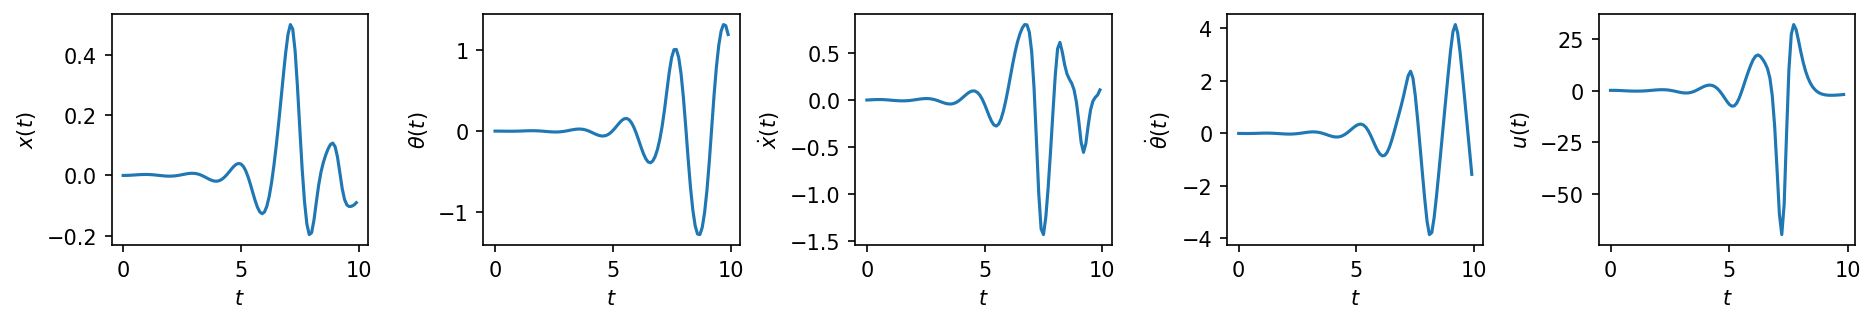
\includegraphics[width=\textwidth]{figures/cartpole_swingup_ol.png}
% \caption{Open-loop application of the iLQR control sequence.}
% \end{figure}

% \begin{figure}[H]
% \centering
% 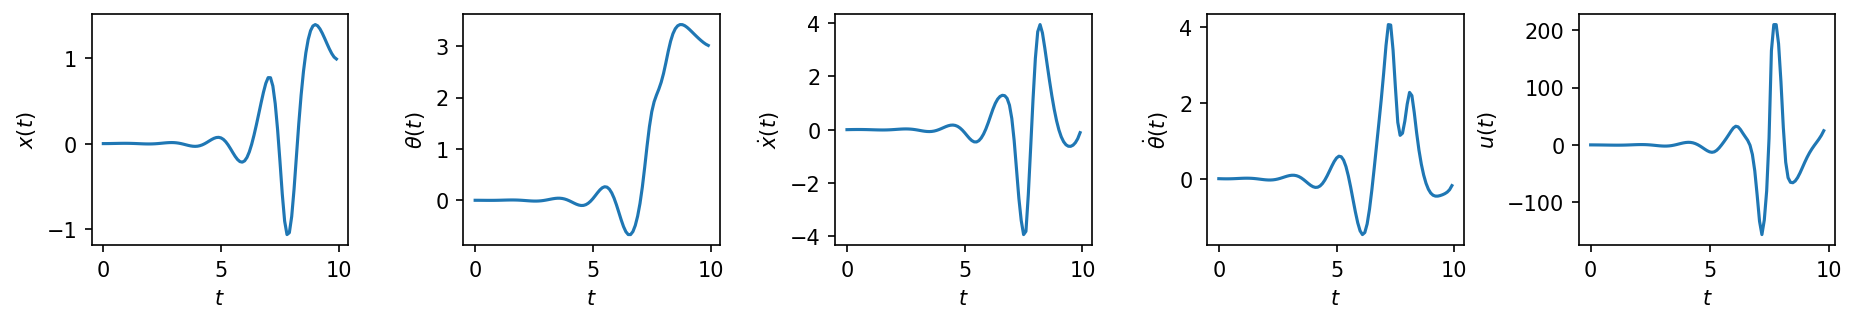
\includegraphics[width=\textwidth]{figures/cartpole_swingup_cl.png}
% \caption{Closed-loop iLQR policy.}
% \end{figure}
